\documentclass{article}

\usepackage{tikz}
\usepackage{pgfplots}
\usepackage{etoolbox}

\title{\Huge\bf Learning Data Plotting}
\date{}

\setlength\oddsidemargin{0pt}

%% Setting a consistent Vertical Space between tikz envs	using 'Environment Hooks' of etoolbox pkg.
\AfterEndEnvironment{tikzpicture}{\vspace{1cm}}

\pgfplotsset{
	tick align=outside, 
	xlabel style={yshift=-5pt},
	compat=1.18,%to get the correct stacking order and alignment of the bars
	colormap={scattermap}{
		color=(teal) color=(yellow) 
		color=(orange) color=(green)
	}
} 
			 
\pgfplotscreateplotcyclelist{scattercycle}{
  {red,  mark=*}, {blue, mark=square*},
  {black, mark=triangle*}
}
\begin{document}
	\maketitle
	
	\section{The axis Environment}
	\begin{tikzpicture} % Line plots
	\begin{axis}[width=10cm,height=6cm]
		\addplot[draw=blue]
			coordinates {(0,0) (1,1) (1,2) (3,0)};
			\addlegendentry{Plot 1}
	\end{axis}
	\end{tikzpicture}  
	
	{\centering
	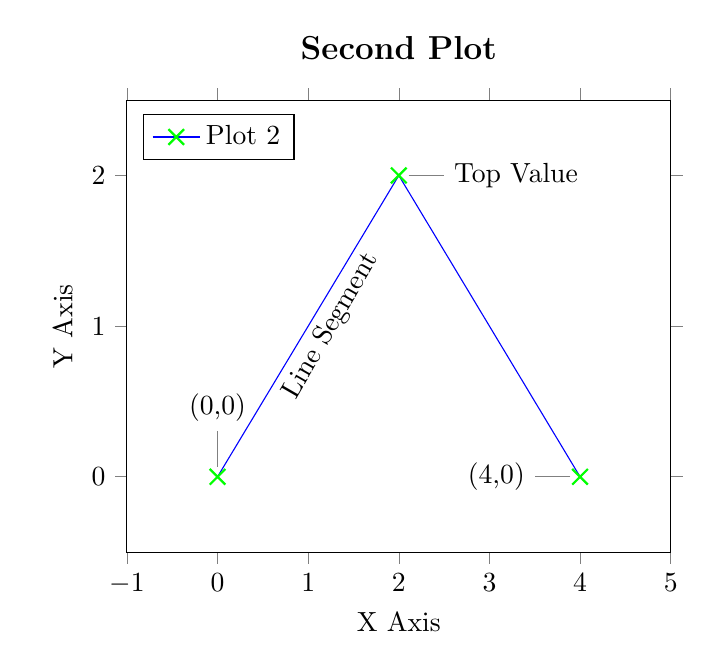
\begin{tikzpicture}
	\begin{axis}[xlabel=X Axis, ylabel=Y Axis, 
					title={\large\bf Second Plot},
					title style={yshift=5pt},
					legend pos=north west,
					enlargelimits=0.25,
					width=0.7\linewidth]
		\addplot[draw=blue,mark=x,mark size=4pt,
				 mark options={thick,green}]
			coordinates {(0,0) (2,2) (4,0)};
		\addlegendentry{Plot 2}
		%% Nodes Incorporating
		\node[pin=right:{Top Value}] 
				at (axis cs: 2,2) {};
		\node[pin=left:{(4,0)}] 
				at (axis cs: 4,0) {};
		\node[pin=above:{(0,0)}] 
				at (axis cs: 0,0) {}; 
		% axis cs is a must to use the axis env 				    coordinate system.
		\node[rotate=60] at (axis cs: 1.25,1) 
				{Line Segment};
	\end{axis}
	%%% Adding a Second Axis env 
	\hspace{9cm}
	\begin{axis}[
				 width=0.7\linewidth,
	             axis lines = left,
   			     xlabel = \(x\),
                 ylabel = \(f(x)\),
                 ymax = 40,
                 %Legend Options
                 legend style={
                 font={\huge},at={(axis cs:1,25)}
                 	}
                 ]
		\addplot[blue,samples=100,domain=-6:6] {x^2};
		\addlegendentry{\(x^2\)}
	\end{axis}
	\end{tikzpicture}
	} 
	%%%%%%%%%%%%%%%%%%%%%%%%%%%%%%%%%%%%%%%%%%%%%%
	%%%%%%%%%%%%%%%%%%%%%%%%%%%%%%%%%%%%%%%%%%%%%%
	
	\section{Bar Graphs}
	
	\subsection{Horizontal Bar Graphs}
	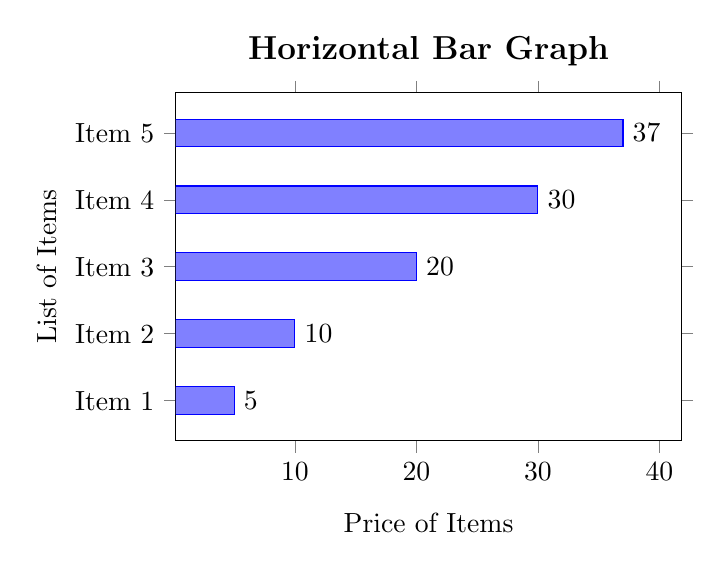
\begin{tikzpicture}
	\begin{axis}
			[xbar, width=8cm,height=6cm,
			 enlargelimits=0.15, 
			 title={\large\bf Horizontal Bar Graph},
			 xlabel={Price of Items},
			 xlabel style={yshift=-5pt},
			 ylabel={List of Items},
			 xtick={0,10,...,40}, ytick={1,2,...,5},
			 yticklabels={Item 1,Item 2,Item 3,
			 				Item 4,Item 5},
			 nodes near coords]
		\addplot[draw=blue, fill=blue!50] coordinates
			{(5,1) (10,2) (20,3) (30,4) (37,5)};
	\end{axis}
	\hspace{8.5cm}
	\begin{axis}[ 
			    xbar, width=8cm,height=6cm,
			    enlargelimits=0.15,
			    symbolic y coords={A, B, C, D, E},
			    ytick=data,
			    xmin=1,xmax=5,
			    xlabel={Numercial Value},
			    ylabel={Category},
			    title={\large\bf Symbolic xbar Graph},
			    nodes near coords
			    ]
		\addplot[draw=red, fill=red!50] coordinates {
		    (4.2,A) (2.4,B) (1.5,C)
		    (3.7,D) (2.1,E)
		};
	\end{axis}
	\end{tikzpicture}	
	
	\subsection{Paired Bar Graphs}
	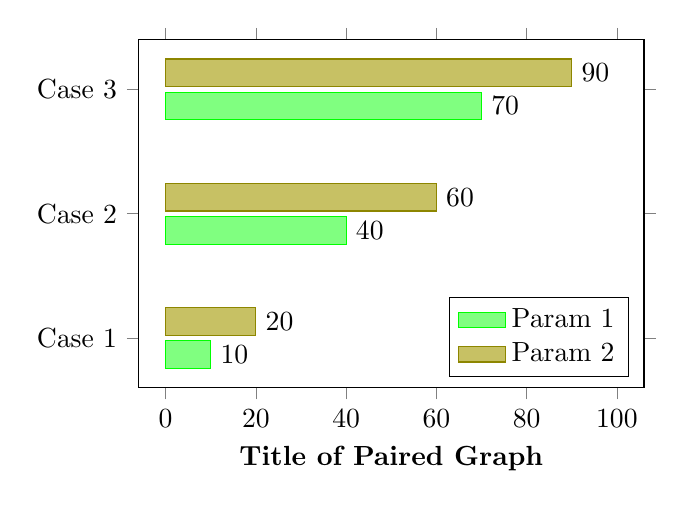
\begin{tikzpicture}
	\begin{axis}[
			 xbar, width=8cm,height=6cm,
			 enlargelimits=0.2,
			 xlabel={\bf Title of Paired Graph},
			 xtick={0,20,...,100}, ytick={1,2,3},
			 yticklabels={Case 1, Case 2, Case 3},
			 % Legend Settings
			 area legend, legend pos=south east,
			 nodes near coords
			 ]
		\addplot[draw=green, fill=green!50]
			coordinates {(10,1) (40,2) (70,3)};
			\addlegendentry{Param 1}
		\addplot[draw=olive, fill=olive!50]
			coordinates {(20,1) (60,2) (90,3)};
			\addlegendentry{Param 2}
	\end{axis}
	\hspace{8.5cm}
	\begin{axis}[
			 xbar, width=8cm,height=6cm,
			 enlargelimits=0.25,
			 xlabel={\bf Title of Paired Graph},
             symbolic y coords={Case 1, Case 2, Case 3},
             ytick=data,
			 % Legend Settings
			 area legend, legend pos=south east,
			 nodes near coords
			 ]
		\addplot[fill=black] coordinates 
			{(10,Case 1) (40,Case 2) (70,Case 3)};
			\addlegendentry{Param 1}
		\addplot[fill=black!50] coordinates 
			{(20,Case 1) (60,Case 2) (90,Case 3)};
			\addlegendentry{Param 2}
	\end{axis}
	\end{tikzpicture}	
	
	\subsection{Stacked Bar Graphs} 
	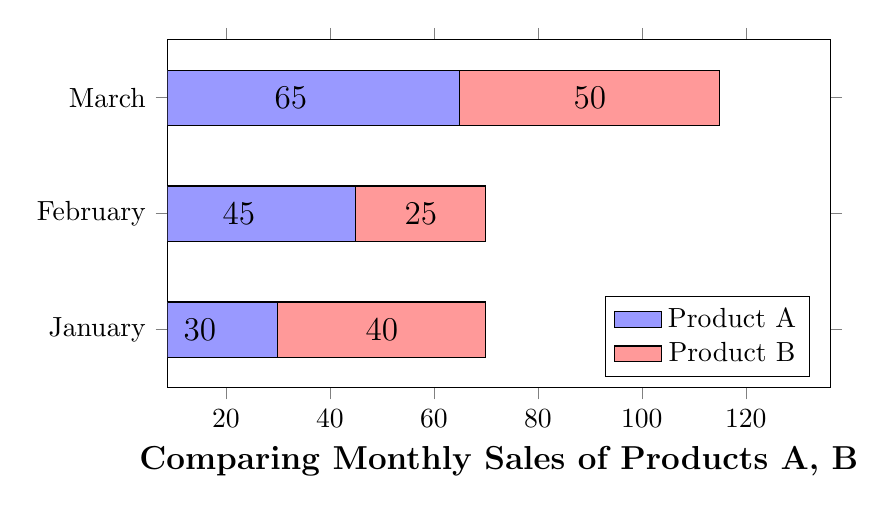
\begin{tikzpicture}
	\begin{axis} % put compat=1.18 in \pgfplotsset
			[
			 xbar stacked, bar width=20pt,
			 % regular stuff
			 height=6cm,width=10cm, enlargelimits=0.25, 
			 nodes near coords,
			 nodes near coords style={font=\large},
			 area legend, legend pos=south east,
			 xlabel={\large\bf Comparing Monthly Sales 						of Products A, B},
			 % tick settings
			 xtick={0,20,...,200}, ytick={1,2,...,5},
			 yticklabels={January, February, March}
			]
		% Product A -- (X, Y) = (Sales<A>, in <Month>)
		\addplot[fill=blue!40] coordinates
			{(30,1) (45,2) (65,3)};
			\addlegendentry{Product A}
		% Product B
		\addplot[fill=red!40] coordinates
			{(40,1) (25,2) (50,3)};
			\addlegendentry{Product B}
	\end{axis}
	\end{tikzpicture}
	
	\subsection{Creating Histogram}
	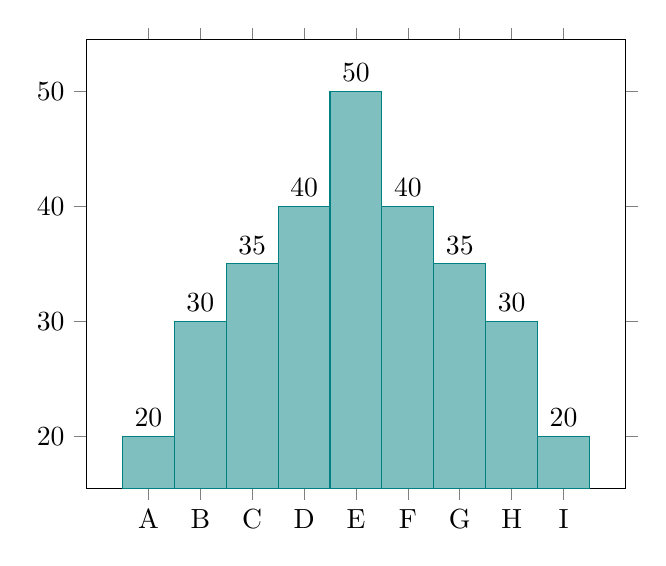
\begin{tikzpicture}
        \begin{axis}[
            ybar, bar width = 1, % width 1 for hist like
            enlargelimits=0.15,
            xtick=data,
            xticklabels={A,B,C,D,E,F,G,H,I},
            nodes near coords
            ]
        \addplot[draw=teal,fill=teal!50] coordinates { 
            (1,20) (2,30) (3,35) (4,40)
            (5,50) (6,40) (7,35) (8,30)
            (9,20)
        };
        \end{axis}
    \end{tikzpicture}
    
	%%%%%%%%%%%%%%%%%%%%%%%%%%%%%%%%%%%%%%%%%%%%%%%%
	%%%%%%%%%%%%%%%%%%%%%%%%%%%%%%%%%%%%%%%%%%%%%%%%
	
	\section{Scatter Plots}
	
	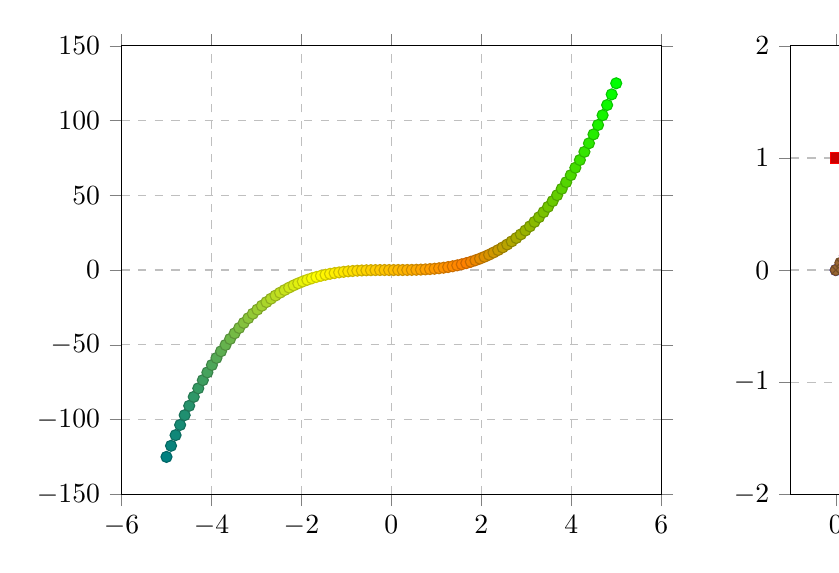
\begin{tikzpicture} 
	\begin{axis}[grid, grid style=dashed]
		\addplot[samples=100, only marks,
				 scatter, scatter src=x,
				 colormap name = scattermap] {x^3};
	\end{axis}
	\hspace{8.5cm}
	\begin{axis}[ymajorgrids=true,grid style=dashed,
  				 legend entries={$sin(x)$,$cos(x)$
  				 	,$tan(x)$},
  				 legend style={at={(axis cs:9,2)}},
  				 ymin=-2, ymax=2]
  		% First default style in cycle list 
    	\addplot+[domain=0:2*pi,only marks,samples=50] 						{sin(deg(x))};
    	% Second default style in cycle list
    	\addplot+[domain=0:2*pi,only marks,samples=50] 						{cos(deg(x))};
    	% Third default style in cycle list
    	\addplot+[domain=0:pi-0.01,only marks,
    		samples=50] {tan(deg(x))};
  	\end{axis}
	\end{tikzpicture}
	
	\begin{tikzpicture}
	% Using the defined cycle list created in preamble
	%% See the pgfplotscreateplotcyclelist
	\begin{axis}[cycle list name = scattercycle,
				 width=12cm, grid, grid style=dashed,
				 legend entries={
				 	$sin(x)+cos(x)$,$cos(x)$,$sin(x)$
				 	}
				 ]
		\addplot+[only marks, samples=100] 
			{sin(deg(x)) + cos(deg(x))};
		\addplot+[only marks, samples=50] 
			{cos(deg(x))};
		\addplot+[only marks, samples=70] 
			{sin(deg(x))};
	\end{axis}
	\end{tikzpicture}
	
	%%%%%%%%%%%%%%%%%%%%%%%%%%%%%%%%%%%%%%%%%%%%%%%%%%
	%%%%%%%%%%%%%%%%%%%%%%%%%%%%%%%%%%%%%%%%%%%%%%%%%%
	
	\section{Reading Data from External File}
	
	\begin{tikzpicture}
	\begin{axis}
		\addplot table {data.txt};
		% Or: \addplot+[only marks] table {data.txt};
	\end{axis}
	\hspace{8cm} 
	\begin{axis} %% [hide axis]
		\addplot[fill=blue!50,line width=2pt] 
			table[x=xCol, y=yCol, col sep=comma]
			{triangle.txt} -- cycle; 
	\end{axis}
	\end{tikzpicture}
	
	%% Histogram example
	\begin{tikzpicture}
	\begin{axis}[
		    ybar, width=12cm, height=9cm, 
		    xmin=0,xmax=200, ymin=0,ymax=2000,
		    axis x line=bottom, axis y line=left,
		    nodes near coords,
		    nodes near coords style = {
		    	black, rotate=90,
		    	anchor = west % drop this to see default
		    },
			xticklabels={2000,...,2018}, 
      		xtick=data,
      		xticklabel style = {rotate=60},
		    xlabel=Years, ylabel=Frequencies,
		    title={\large\bf Frequency Histogram},
		    title style={at={(axis cs:100,2200)}},
		    after end axis/.code={
            \draw [->] % Extend x axis
            	(axis cs:200,0) -- (axis cs:210,0); 
            \draw [->] % Extend y axis
            	(axis cs:0,2000) -- (axis cs:0,2200); 
        	},
        	axis line style={-} 
		]
		\addplot+[fill=blue!30, draw=black] 
		    table[x=YearXLoc, y=Frequency] {hist.txt};
	\end{axis}
	\end{tikzpicture}
	
	\subsection{Combining Multiple Data-sets}
	\begin{tikzpicture}[scale=1.3]
	\begin{axis}[
			DataStyle/.style=
				{mark=square,thick,teal,dashed},
			hide axis
			]
		\addplot[DataStyle] table {data1.txt};
		\addplot[fill=blue!50,line width=2pt] 
			table[x=xCol, y=yCol, col sep=comma]
			{triangle1.txt} -- cycle;
	\end{axis}
	\begin{axis}
		\addplot+ table[x=YearXLoc,y=Frequency] 						{hist.txt};
	\end{axis}
	\end{tikzpicture}
	
	\section{3-D Plotting}
	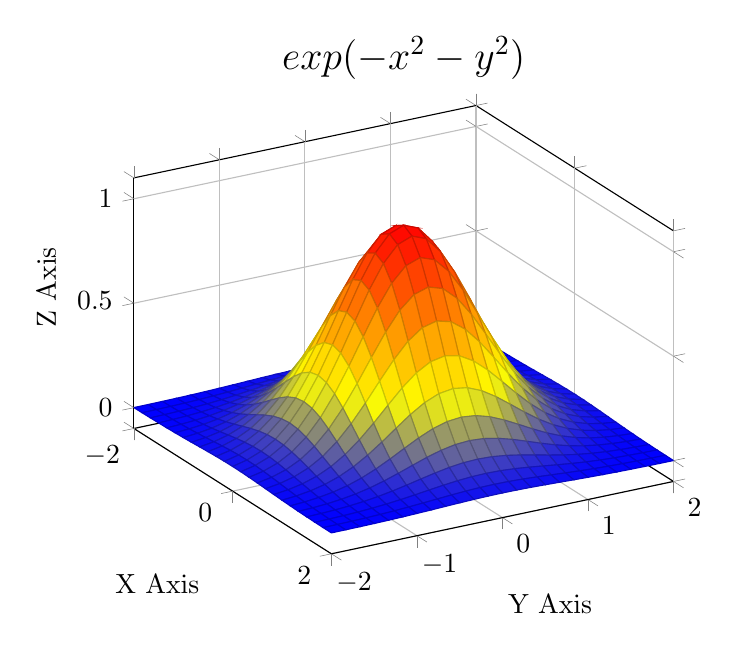
\begin{tikzpicture}
	\begin{axis}[
		xlabel=X Axis, ylabel=Y Axis, zlabel=Z Axis,
		title={\Large \(exp(-x^2-y^2)\)},
		% viewed from an angle of 60 degrees around 			  the x-axis and 30 degrees around the y-axis.
		view={60}{30}, grid=both
		]
		\addplot3[
			surf, colormap/hot, % TRY: cool
			domain=-2:2, domain y=-2:2
		] {exp(-x^2-y^2)};
	\end{axis}
	\end{tikzpicture}
	
\end{document}